\begin{figure}[H]
    \centering
    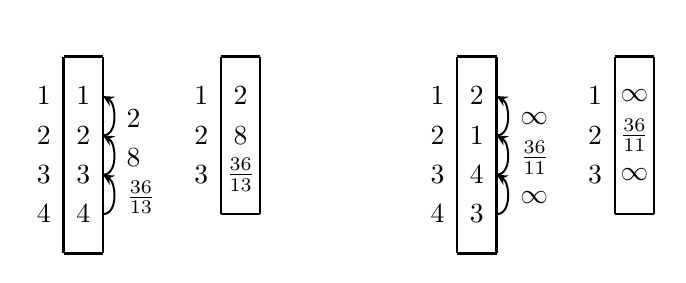
\begin{tikzpicture}[thick]
        \node at (0.5,0 cm) {$4$};
        \node at (0.5,0.5 cm) {$3$};
        \node at (0.5,1 cm) {$2$};
        \node at (0.5,1.5 cm) {$1$};

        \draw (0.75,-0.5) -- (0.75, 2);
        \draw (1.25,-0.5) -- (1.25, 2);
        \draw (0.75,-0.5) -- (1.25,-0.5);
        \draw (0.75, 2) -- (1.25, 2);
        \node at (1,0 cm) {$4$};
        \node at (1,0.5 cm) {$3$};
        \node at (1,1 cm) {$2$};
        \node at (1,1.5 cm) {$1$};

        \draw[->, shorten >= 0.1pt, shorten <= 0.1pt, >=stealth, line width=0.25mm]
        (1.25, 0) to[out=0,in=-30] node[right=1pt] {$\frac{36}{13}$} (1.25, 0.5);

        \draw[->, shorten >= 0.1pt, shorten <= 0.1pt, >=stealth, line width=0.25mm]
        (1.25, 0.5) to[out=0,in=-30] node[right=1pt] {$8$} (1.25, 1);

        \draw[->, shorten >= 0.1pt, shorten <= 0.1pt, >=stealth, line width=0.25mm]
        (1.25, 1) to[out=0,in=-30] node[right=1pt] {$2$} (1.25, 1.5);

        \node at (1,2.25 cm) {$\sorted$};

        \node at (2.5,0.5 cm) {$3$};
        \node at (2.5,1 cm) {$2$};
        \node at (2.5,1.5 cm) {$1$};

        \draw (2.75,0) -- (2.75, 2);
        \draw (3.25,0) -- (3.25, 2);
        \draw (2.75,0) -- (3.25,0);
        \draw (2.75, 2) -- (3.25, 2);
        \node at (3,0.5 cm) {$\frac{36}{13}$};
        \node at (3,1 cm) {$8$};
        \node at (3,1.5 cm) {$2$};

        \node at (3,2.25 cm) {$\cert$};

        \begin{scope}
            [shift={(5,0)}]
            \node at (0.5,0 cm) {$4$};
            \node at (0.5,0.5 cm) {$3$};
            \node at (0.5,1 cm) {$2$};
            \node at (0.5,1.5 cm) {$1$};

            \draw (0.75,-0.5) -- (0.75, 2);
            \draw (1.25,-0.5) -- (1.25, 2);
            \draw (0.75,-0.5) -- (1.25,-0.5);
            \draw (0.75, 2) -- (1.25, 2);
            \node at (1,0 cm) {$3$};
            \node at (1,0.5 cm) {$4$};
            \node at (1,1 cm) {$1$};
            \node at (1,1.5 cm) {$2$};

            \draw[->, shorten >= 0.1pt, shorten <= 0.1pt, >=stealth, line width=0.25mm]
            (1.25, 0) to[out=0,in=-30] node[right=1pt] {$\infty$} (1.25, 0.5);

            \draw[->, shorten >= 0.1pt, shorten <= 0.1pt, >=stealth, line width=0.25mm]
            (1.25, 0.5) to[out=0,in=-30] node[right=1pt] {$\frac{36}{11}$} (1.25, 1);

            \draw[->, shorten >= 0.1pt, shorten <= 0.1pt, >=stealth, line width=0.25mm]
            (1.25, 1) to[out=0,in=-30] node[right=1pt] {$\infty$} (1.25, 1.5);

            \node at (1,2.25 cm) {$\sorted$};

            \node at (2.5,0.5 cm) {$3$};
            \node at (2.5,1 cm) {$2$};
            \node at (2.5,1.5 cm) {$1$};

            \draw (2.75,0) -- (2.75, 2);
            \draw (3.25,0) -- (3.25, 2);
            \draw (2.75,0) -- (3.25,0);
            \draw (2.75, 2) -- (3.25, 2);
            \node at (3,0.5 cm) {$\infty$};
            \node at (3,1 cm) {$\frac{36}{11}$};
            \node at (3,1.5 cm) {$\infty$};

            \node at (3,2.25 cm) {$\cert$};

        \end{scope}
    \end{tikzpicture}
    \caption[Exemplo das estruturas utilizadas na lista ordenada]{Vetores $\sorted$ e $\cert$ para
        $\now = 0$ e $\now = 3$.
        O instante $t = \frac{36}{13}$ é quando as trajetórias dos elementos $3$ e $4$ se cruzam, e
        $t = \frac{36}{11}$ é quando as trajetórias dos elementos $1$ e $4$ se cruzam.}
    \label{fig:lista:variaveis}
\end{figure}

